\section{Auswertung}

\subsection{Bestimmung der Schallgeschwindigkeit in Acryl \label{sec:schall}}

\subsubsection{Impuls-Echo-Verfahren}

In Tabelle \ref{tab:echo} befinden sich die aufgenommenen Messwerte
\begin{table}[H]
   \centering
   \caption{Mithilfe des Impuls-Echo-Verfahrens aufgenommenen Messwerte}
   \label{tab:echo}
   \begin{tabular} { S S S S }
 \toprule
 & {Puls $1$} & {Puls $2$} \\
\cmidrule(lr){2-2} \cmidrule(lr){3-3}
 {$L\:/\: \mathrm{cm}$} & {$U\:/\: \mathrm{V}$} & {$U\:/\: \mathrm{V}$} & {$\symup{\Delta}t\:/\: \mathrm{μs}$} \\
    \midrule
    12,0 & 1,405 & 0,663 & 88,7 \\
    10,2 & 1,405 & 0,646 & 76,4 \\
    8,0 & 1,401 & 1,268 & 59,5 \\
    7,1 & 1,401 & 1,318 & 46,5 \\
    6,2 & 1,417 & 1,396 & 46,3 \\
    4,0 & 1,401 & 1,446 & 29,4 \\
    3,1 & 1,392 & 1,355 & 23,6 \\
    \bottomrule
  \end{tabular}
\end{table}


In Graph \ref{fig:echo} sind diese aufgetragen.
\begin{figure}[H]
  \centering
  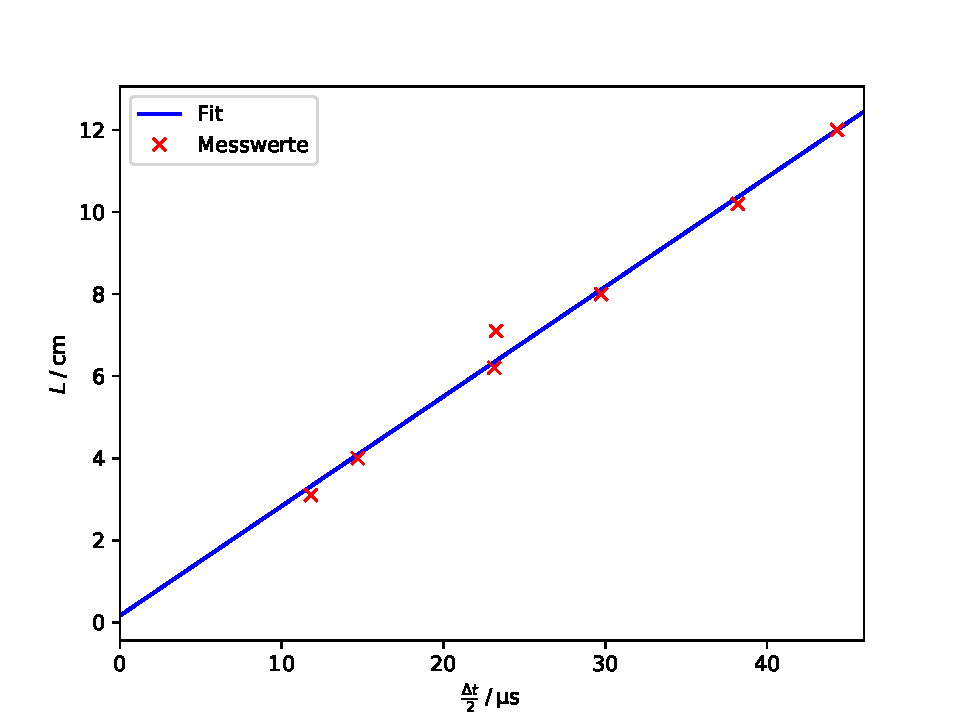
\includegraphics[width=\textwidth]{Plots/echo.pdf}
  \caption{Es ist die Länge des Acrylzylinders $L$ gegen die Zeit $\sfrac{\symup{\Delta}t}{2}$, die der Schall benötigt um diesen beim Impuls-Echo-Verfahren einmal zu durchqueren, aufgetragen.}
  \label{fig:echo}
\end{figure}

Eine lineare Regression $f(x) = a \cdot x + b$ liefert die Werte
\begin{align*}
  a &= \SI{2669,59(12355)}{\m \per \s} = c_\text{Echo} \\
  b &= \SI{0,17(35)}{\cm}.
\end{align*}

Dabei ist die Steigung $a$ die Geschwindigkeit, mit der sich der Schall durch Acryl bewegt und der y-Achsenabschnitt $b$ ist
die Dicke der Anpassungsschicht.
Der Theoriewert \cite{sample2} ist $c_\text{Acryl, theo} = \SI{2730}{\m \per \s}$, die Abweichung beträgt $\SI{2,21}{\%}$.

\subsubsection{Durchschallungs-Verfahren}

In Tabelle \ref{tab:durch} befinden sich die aufgenommenen Messwerte
\begin{table}[H]
   \centering
   \caption{Mithilfe des Durchschallungs-Verfahrens aufgenommenen Messwerte}
   \label{tab:durch}
   \begin{tabular} { S S }
 \toprule
 {$L\:/\: \mathrm{cm}$} & {$\symup{\Delta}t\:/\: \mathrm{μs}$} \\
    \midrule
    12,0 & 45,7 \\
    10,2 & 39,2 \\
    8,0 & 31,4 \\
    7,1 & 27,7 \\
    6,2 & 23,8 \\
    4,0 & 15,7 \\
    3,1 & 12,4 \\
    \bottomrule
  \end{tabular}
\end{table}


Aufgetragen sind diese in Graph \ref{fig:durch}.
\begin{figure}[H]
  \centering
  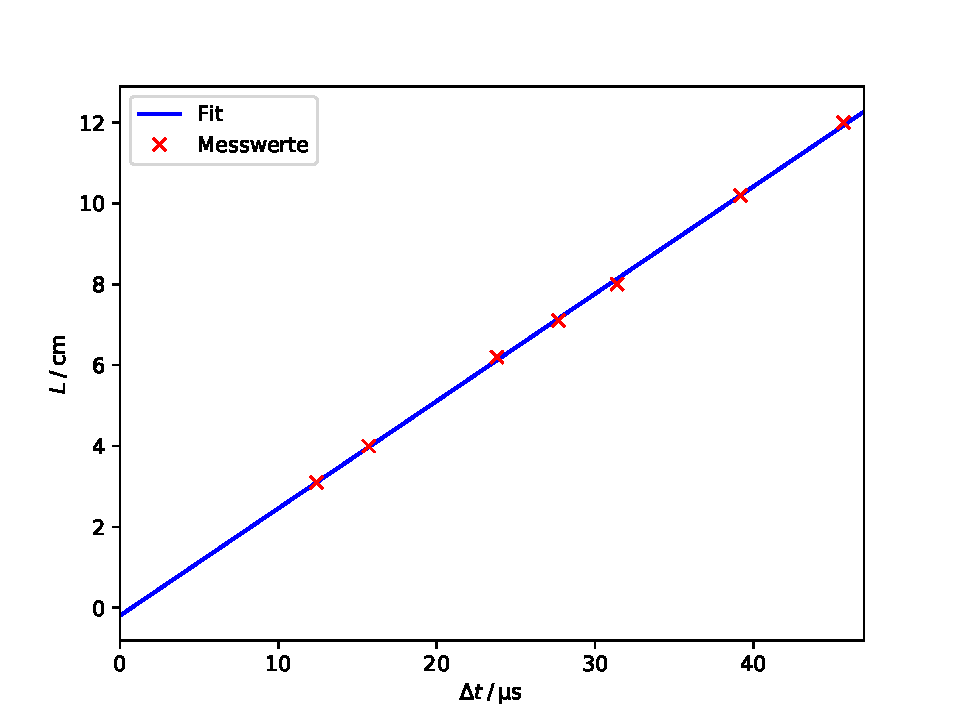
\includegraphics[width=\textwidth]{Plots/durch.pdf}
  \caption{Es ist die Länge des Acrylzylinders $L$ gegen die Zeit $\symup{\Delta}t$, die der Schall benötigt um diesen beim Durchschallungs-Verfahren einmal zu durchqueren, aufgetragen.}
  \label{fig:durch}
\end{figure}

Eine lineare Regression $f(x) = a \cdot x + b$ liefert die Werte
\begin{align*}
  a &= \SI{2652,62(2796)}{\m \per \s} = c_\text{Durch} \\
  b &= \SI{-0,19(8)}{\cm}.
\end{align*}

Dabei ist die Steigung $a$ wieder die Geschwindigkeit, mit der sich der Schall durch Acryl bewegt und der y-Achsenabschnitt $b$ ist
die Dicke der Anpassungsschicht. Die Abweichung zum Theoriewert \cite{sample2} beträgt $\SI{2,83}{\%}$.

Der Mittelwert beträgt
\begin{equation*}
  \bar{c}_\text{Acryl} = \frac{c_\text{Echo}+c_\text{Durch}}{2} = \SI{2661,10(6334)}{\m \per \s}.
\end{equation*}

Der Fehler ergibt sich aus der Gauß'schen Fehlerfortpflanzung
\begin{equation*}
  \sigma_{\bar{c}_\text{Acryl}} = \sqrt{\left( \frac{1}{2} \sigma_{c_\text{Echo}} \right)^2 + \left( \frac{1}{2} \sigma_{c_\text{Durch}} \right)^2}
\end{equation*}

Der Mittelwert weicht um $\SI{2,52}{\%}$ vom Theoriewert \cite{sample2} ab.

\subsection{Bestimmung des Dämpfungskoeffizienten mithilfe des Impuls-Echo-Verfahrens \label{sec:daem}}

In Abbildung \ref{fig:däm} sind die Werte aus Tabelle \ref{tab:echo} aufgetragen.
\begin{figure}[H]
  \centering
  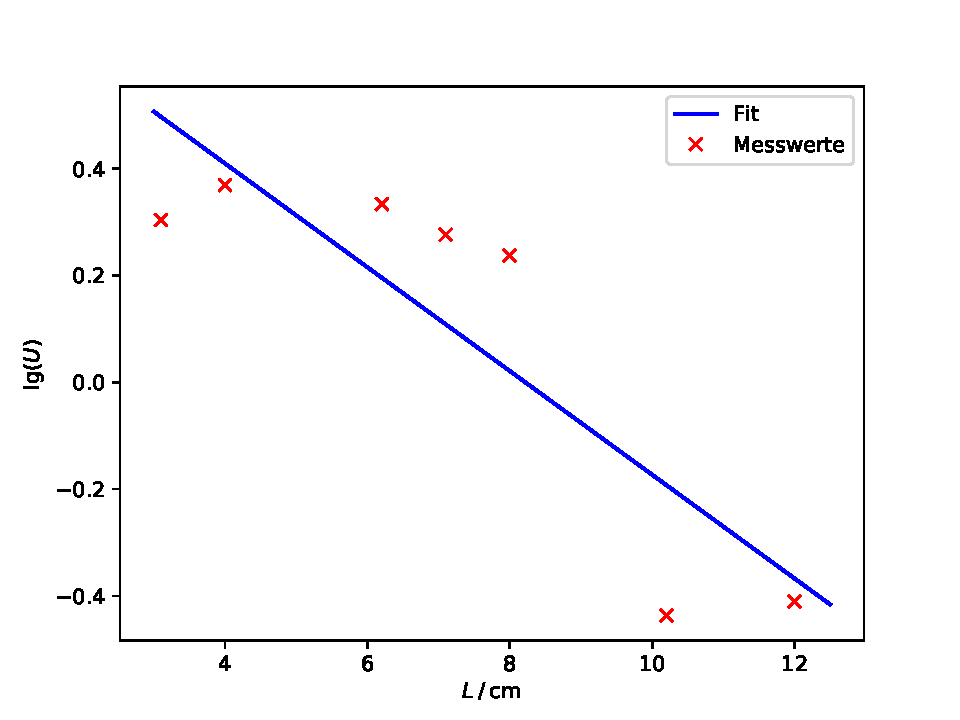
\includegraphics[width=\textwidth]{Plots/daem.pdf}
  \caption{$\ln{(U)}$-$L$-Diagramm zur Bestimmung des Dämpfungskoeffizienten}
  \label{fig:däm}
\end{figure}

Eine lineare Regression $f(x) = -a \cdot x + b$ liefert folgende Werte
\begin{align*}
  a &= \SI{-9,71(28)}{\per \m} = - \alpha \\
  b &= \SI{0,8(2)}{}.
\end{align*}

Der Dämpfungsfaktor in Acryl ist somit $\alpha = \SI{9,71(28)}{\per \m}$. Der Theoriewert \cite{sample4} beträgt $\alpha_\text{theo} = \SI{57}{\per \m}$,
wodurch sich eine Abweichung von $\SI{82,96}{\%}$ ergibt.

\subsection{Bestimmung der Dicke zweier Acrylplatten mithilfe des Cepstrums und des A-Scans \label{sec:cep}}

Die aufgenommenen Messwerte befinden sich in Tabelle \ref{tab:cep}.
\begin{table}[H]
   \centering
   \caption{Aus dem Cepstrum und A-Scan bestimmte Laufzeiten durch zwei Acrylplatten}
   \label{tab:cep}
   \begin{tabular} { c S S }
 \toprule
  & {$\symup{\Delta}t_\text{Cep} \:/\: \mathrm{μs}$} & {$\symup{\Delta}t_\text{Scan}\:/\: \mathrm{μs}$} \\
    \midrule
    $\symup{\Delta}t_1$ & 4,90 & 4,8 \\
    $\symup{\Delta}t_2$ & 8,74 & 8,6 \\
    $\symup{\Delta}t_3$ & 13,21 & 13,4 \\
    \bottomrule
  \end{tabular}
\end{table}


In Abbildung \ref{fig:cep} sind Das FTT und das Cepstrum zu sehen.
\begin{figure}[H]
  \centering
  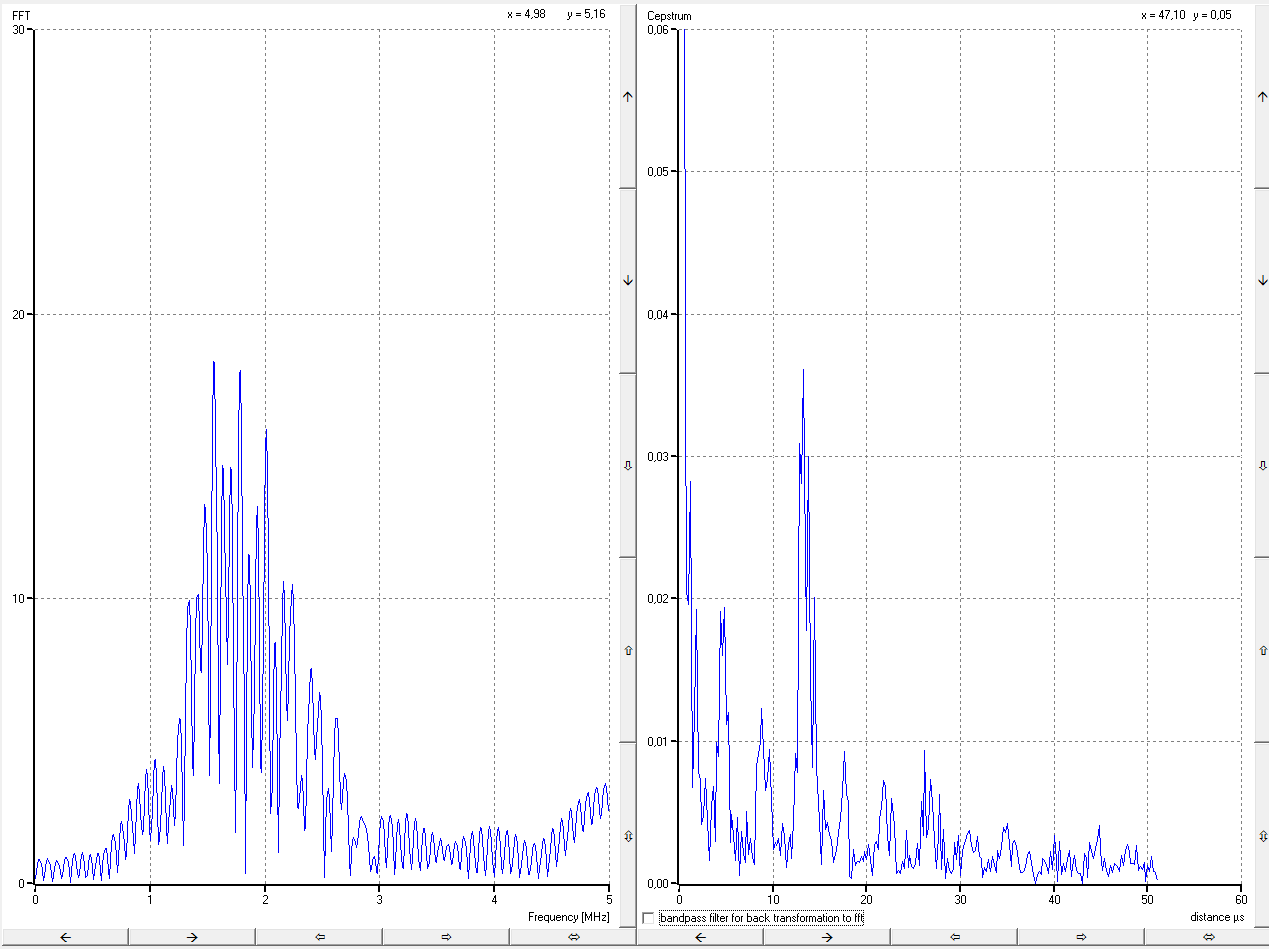
\includegraphics[width=\textwidth]{Text/Bilder/FTT,Cep.png}
  \caption{Screenshot des aufgenommenen FTT und Cepstrum}
  \label{fig:cep}
\end{figure}

Aus den gemessenen Laufzeiten werden nun die Dicken der einzelnen Platten und deren Gesamtdicke nach Gleichung \eqref{eqn:dicke} berechnet.
\begin{equation}
  d = \frac{\symup{\Delta}t}{2} \bar{c}_\text{Acryl}
  \label{eqn:dicke}
\end{equation}

Für die aufgenommenen Zeiten ergibt sich:
\begin{align*}
  d_{1, \text{Cep}} &= \SI{0,652(16)}{\cm} & d_{1, \text{Scan}} &= \SI{0,639(15)}{\cm} \\
  d_{2, \text{Cep}} &= \SI{1,163(28)}{\cm} & d_{2, \text{Scan}} &= \SI{1,144(27)}{\cm} \\
  d_{3, \text{Cep}} &= \SI{1,76(4)}{\cm} & d_{3, \text{Scan}} &= \SI{1,78(4)}{\cm}
\end{align*}

Die Mittelwerte und ihre Fehler ergeben sich aus den Gleichungen \eqref{eqn:dmit} und \eqref{eqn:derr}.
\begin{align}
  \bar{d} &= \frac{d_\text{Cep} + d_\text{Scan}}{2} \label{eqn:dmit} \\
  \sigma_{\bar{d}} &= \sqrt{\frac{1}{1 \cdot 2}  \left((\bar{d}-d_\text{Cep})^2+(\bar{d}-d_\text{Scan})^2 \right)} \label{eqn:derr}
\end{align}

Die Mittelwerte sind somit
\begin{align*}
  \bar{d}_1 &= \SI{0,645(15)}{\cm} \\
  \bar{d}_2 &= \SI{1,154(27)}{\cm} \\
  \bar{d}_3 &= \SI{1,77(4)}{\cm}.
\end{align*}

Die Abweichungen von den mithilfe der Schiebelehre bestimmten Werte
\begin{align*}
  d_{1, \text{theo}} &= \SI{0,6}{\cm} \\
  d_{2, \text{theo}} &= \SI{1,2}{\cm} \\
  d_{3, \text{theo}} &= \SI{1,8}{\cm}
\end{align*}

liegen bei $\SI{7,55}{\%}$ für $ d_1$, $\SI{3,87}{\%}$ für $d_2$ und $\SI{1,65}{\%}$ für $d_3$.

\subsection{Biometrische Untersuchung eines Augenmodells}

Die aufgenommenen Messwerte befinden sind
\begin{align*}
  \symup{\Delta}t_1 = 12,\!1 \: \symup{\mu s} \\
  \symup{\Delta}t_2 = 17,\!8 \: \symup{\mu s} \\
  \symup{\Delta}t_3 = 26,\!9 \: \symup{\mu s} \\
  \symup{\Delta}t_4 = 70,\!5 \: \symup{\mu s} \\
\end{align*}

Die jeweiligen Schallgeschwindigkeiten betragen
\begin{align*}
  c_\text{K} &= \SI{1483}{\m \per \s} \\
  c_\text{L} &= \SI{2500}{\m \per \s} \\
  c_\text{GK} &= \SI{1410}{\m \per \s}.
\end{align*}

Dabei ist $c_\text{L}$ die Schallgeschwindigkeit in der Linse \cite[6]{sample}, $c_\text{GK}$ die Schallgeschwindigkeit im Glaskörper \cite[6]{sample}
und $c_\text{K}$ die Schallgeschwindigkeit in der vorderen und hinteren Augenkammer, die mit der Schallgeschwindigkeit für Wasser \cite{sample3}
angenähert wird.

Die berechneten Werte sind:
\begin{align*}
  &\text{Hornhaut - Iris:} &d_1 &= \frac{\symup{\Delta}t_1}{2} c_\text{K} = \SI{0,90}{\cm} \\
  &\text{Iris - Linsenanfang:} &d_2 &= \frac{\symup{\Delta}t_2}{2} c_\text{K} = \SI{0,42}{\cm} \\
  &\text{Linsenanfang - Linsenende:} &d_3 &= \frac{\symup{\Delta}t_3}{2} c_\text{L} = \SI{1,14}{\cm} \\
  &\text{Linsenende - Retina:} &d_4 &= \frac{\symup{\Delta}t_4}{2} c_\text{GK} = \SI{3,07}{\cm}.
\end{align*}
